
Here is the third analysis iteration, the heavyweight version of the RQ2 experiment, run in a current scene-graph framework against three predictions registered before it (\S{}6.1). It reaches a different verdict from Chapter 5, and \S{}6.4 works out why.

\section{Design}

In Chapter 5 the controlled experiment used a deliberately small classifier. Here the heavyweight version runs at the scale the field measures, using a real-time scene-graph model, REACT++, which is the current model of the open SGG-Benchmark framework (Neau and Falomir, 2026), trained once on the human relations and once on this tool's, then evaluated on an identical held-out test set. The source paper benchmarked a different set of relation models, VCTree scoring best among them (\S{}2.6), so this is its task, split and metrics run with a current model, not a re-run of its configuration. The isolation mirrors RQ2 exactly:

\begin{itemize}
\item \textbf{Shared detector.} A YOLOv8m backbone is trained once on the ground-truth boxes of the training split and frozen for both arms (test-time detection mAP is bit-identical between arms: 0.654). The relation labels are the intended difference. There is one other the design does not remove: each arm's best checkpoint is chosen on validation scored against its \textit{own} labels (\S{}6.2), so the two arms are selected under different objectives before they meet the common human test gold. A cleaner design would fix the epoch in advance or select on a shared target, and the comparison should be read as label source plus selection rule rather than label source alone.
\item \textbf{Split} follows the calibration protocol: train = groups 0--4 (500 images; 5,421 human vs 119,020 automatic relations; the 22$\times$ density difference is the treatment), validation = group 5, test = groups 6--8 (human gold in both arms; the framework's loader retains 210 of the 236 test images).
\item \textbf{Three predictions were registered in \S{}5.6 before the run}: (1) the human-label arm saturates early, replicating the source paper; (2) the auto-label arm reaches a higher plateau; (3) \texttt{near} recovers.
\end{itemize}

\section{Training dynamics: prediction 1 confirmed}

Peaking at \textbf{epoch 4 of 25}, the human arm never improves again, oscillating between 0.101 and 0.122 for the remaining twenty-one, which is mild overfitting on 5,421 sparse triplets. That reproduces the source paper's central observation ("all predictors reached their peak mR@100 well before the final epoch") with a current model, and it adds the cause, which is that sparse supervision gets exhausted early. Still climbing at epoch 8, the auto arm does not reach 95\% of its best until \textbf{epoch 14} and peaks at \textbf{epoch 22}, and sees 213 distinct triplet types in training against 94 for the human arm. Figure~\ref{fig:sgg-training-curves} plots both. Each validation series uses its own arm's labels, so only the \textit{shapes} compare.
\begin{figure}[!htbp]
\centering
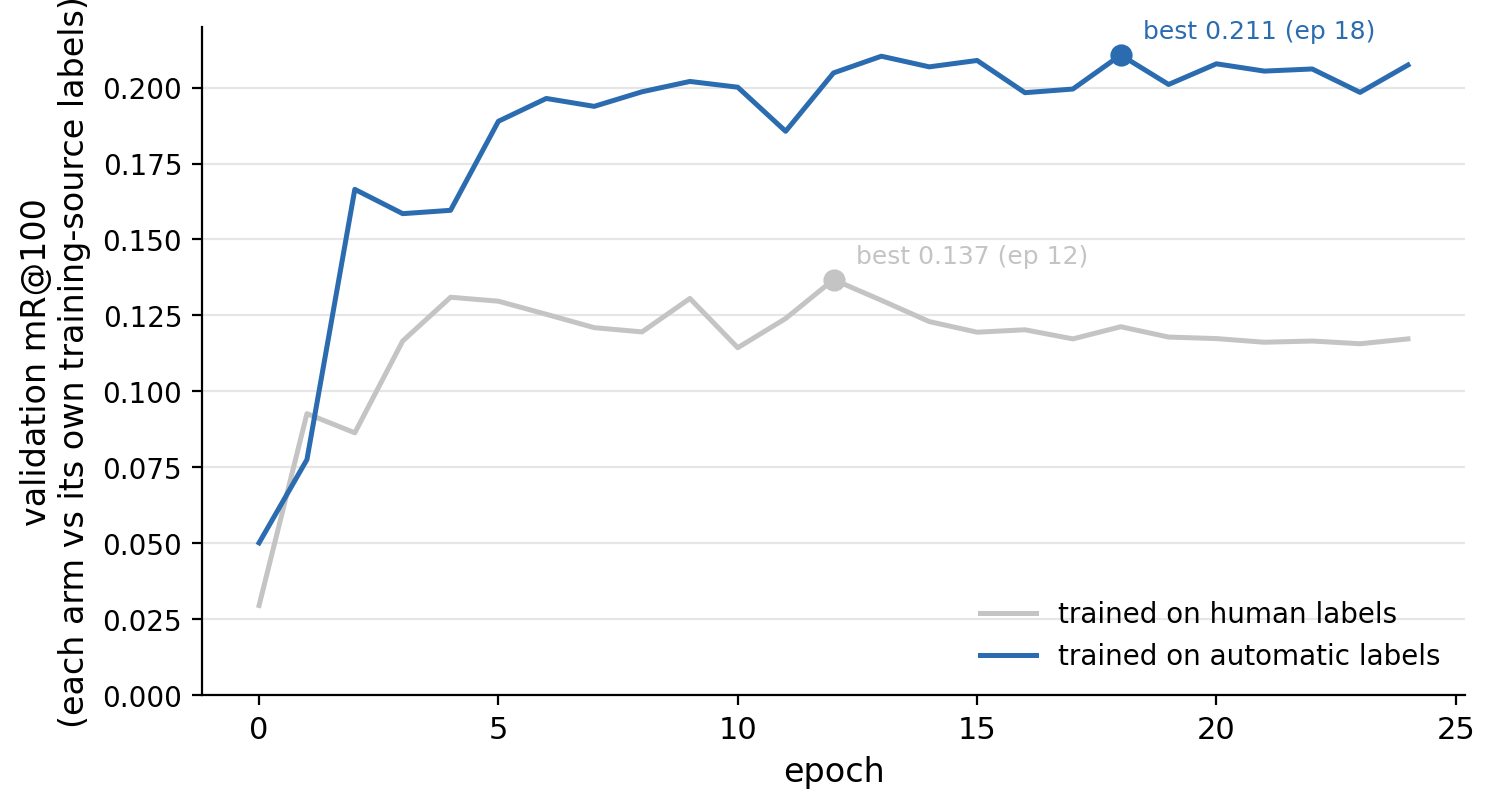
\includegraphics[width=0.80\textwidth,height=0.78\textheight,keepaspectratio]{figures/sgg-training-curves.png}
\caption[Validation curves for both benchmark arms]{Validation curves for both benchmark arms, each against its own training-source labels, so only the shapes are comparable. The human arm peaks early and declines; the automatic arm does not.}
\label{fig:sgg-training-curves}
\end{figure}


\section{Test results: prediction 2 unresolved, prediction 3 refuted}

Both best checkpoints, evaluated on the identical test set of 210 images with human gold from groups 6--8, at seed 42:

\needspace{9.7\baselineskip}
\begin{center}
\setlength{\tabcolsep}{3pt}
\footnotesize
\begin{longtable}{lll}
\caption[Benchmark test results (SGDet) for the human-trained]{Benchmark test results (SGDet) for the human-trained and auto-trained arms, at seed 42; Table 6.2 pools all three seeds.}\\
\hline
metric (test, sgdet) & human-trained & auto-trained \\
\hline
\endfirsthead
\hline
metric (test, sgdet) & human-trained & auto-trained \\
\hline
\endhead
R@100 & \textbf{0.280} & 0.259 \\
mR@100 & 0.270 & \textbf{0.291} \\
F1@100 & \textbf{0.275} & 0.274 \\
zR@100, recall on types the shared reference omits (\S{}6.4) & 0.073 & \textbf{0.309} \\
\hline
\end{longtable}
\end{center}

At this seed the automatic arm leads on mean recall, 0.291 against 0.270, while the human arm keeps raw recall and the two come out level on F1. Predicate by predicate, the ordering inverts. Five of the seven go to the human arm, with the automatic arm ahead on the support pair, by 0.077 on \texttt{on} and 0.284 on \texttt{under}. For \texttt{near} both arms sit far below the source paper's 0.22--0.25 floor, 0.117 and 0.108, so prediction 3 is refuted as stated. Its dense, fitted \texttt{near} does not survive the trip through a learned model.

Sharpest of all is the separation on triplet \textit{types never seen in training}, 0.309 against 0.073, fourfold at this seed and fivefold over three (\S{}6.3.1). Section 6.4 sets out what that column measures here, coverage of relation types the manual annotation never recorded, not compositional generalisation. Prediction 2 is the one a single run cannot carry in either direction, with the margin sitting well inside the human arm's own seed spread. That is why \S{}6.3.1 exists. Supplementary F.1 carries the per-predicate and per-slice breakdown, and aligning the front/behind convention of groups 6 and 8, one disclosed bit per group as in \S{}4.5, lifts both arms and leaves them level, 0.310 against 0.312.

\subsection{Replication across seeds, and one claim withdrawn}

Two of those margins are far too small for one run to separate from training noise. Both arms were retrained at seeds 43 and 44 and all six checkpoints re-scored on every slice (\texttt{scripts/kaggle/}, aggregated by \texttt{eval/seed\_\allowbreak{}stats.py}) against the same frozen detector, so the spread below is the relation model's own variance.

\needspace{12.8\baselineskip}
\begin{center}
\setlength{\tabcolsep}{2pt}
\footnotesize
\begin{longtable}{lllrrl}
\caption[Seed replication]{Seed replication: which differences separate across three seeds per arm.}\\
\hline
slice & metric & conv. & human-trained & auto-trained & vision-language \\
\hline
\endfirsthead
\hline
slice & metric & conv. & human-trained & auto-trained & vision-language \\
\hline
\endhead
full test & mR@100 & mixed & 0.293 (0.270--0.322) & 0.292 (0.290--0.296) & \textbf{0.329} (0.312--0.357) \\
full test & zR@100 & mixed & 0.052 (0.004--0.079) & 0.268 (0.225--0.309) & \textbf{0.307} (0.256--0.371) \\
group 6 & mR@100 & \textbf{inv.} & 0.327 (0.299--0.364) & 0.305 (0.296--0.312) & \textbf{0.337} (0.316--0.366) \\
group 6 & zR@100 & inv. & 0.000 (0.000--0.000) & \textbf{0.449} (0.348--0.530) & 0.202 (0.086--0.343) \\
group 7 & mR@100 & clean & 0.278 (0.254--0.298) & 0.289 (0.280--0.300) & \textbf{0.362} (0.357--0.364) \\
group 7 & zR@100 & clean & 0.098 (0.008--0.148) & 0.273 (0.234--0.346) & \textbf{0.456} (0.433--0.496) \\
group 8 & mR@100 & \textbf{inv.} & 0.147 (0.130--0.164) & 0.120 (0.108--0.131) & \textbf{0.164} (0.146--0.183) \\
group 8 & zR@100 & inv. & 0.007 (0.000--0.013) & 0.041 (0.033--0.048) & \textbf{0.090} (0.038--0.117) \\
aligned & mR@100 & corrected & 0.333 (0.310--0.369) & 0.316 (0.312--0.320) & \textbf{0.369} (0.354--0.390) \\
\hline
\end{longtable}
\end{center}

I trained all nine runs in one session, on one clone, one frozen detector and one configuration, so the arms differ in their labels and nothing else. Earlier figures, with the human arm at 0.326 pooled, came from runs made weeks apart against different states of the upstream code, and \S{}7.4 reports what that cost. In the \textbf{aligned} row the same models are re-scored against gold with the two inverted annotators corrected (\S{}4.5). The \texttt{zR@100} rows measure coverage of types omitted from one shared reference (\S{}6.4), and this dissertation makes no zero-shot claim on them.

\textbf{On the metric this chapter is organised around, the two label sources are indistinguishable.} Every row's seed ranges overlap, and paired by seed the automatic arm leads at 42 (+0.021) and 43 (+0.010) and trails at 44 (-0.032), so the pooled difference of 0.001 rests on a single run. Parity is the correct statement, and it is about this metric, not about the labels, since on raw R@100 the human arm keeps a real margin pooled, 0.295 against 0.255, and on zero-shot recall the automatic arm leads fivefold, 0.268 against 0.052. Stability, not score, is where the arms really differ. Pooled mR@100 for the automatic arm spans 0.006 across seeds against the human arm's 0.052, so one definition applied uniformly lands in the same place whatever the initialisation, and nine annotators applying nine conventions do not.

Where the arms do differ, they differ by annotator. On the two groups \S{}4.5 convicts of inverting the convention the human arm leads, and it \textit{trails} on group 7, the one convicted of nothing, so the ordering runs with annotation quality, not with geometry. Supplementary F.9 gives the three margins, none separable across seeds, the contamination behind them (\textbf{30\% of the entire yardstick is front/behind written by the two inverted annotators}, a shared ceiling, not a differential), and the replication at the earlier \texttt{on\_\allowbreak{}contact\_\allowbreak{}min} 0.60 under which the same ordering holds. Every absolute figure in this chapter is therefore a lower bound. Both sides pay it.

Second, \textbf{the zero-shot result is robust and larger than first reported.} Pooled zR@100 is 0.268 against 0.052, roughly fivefold, with disjoint ranges. It is not an artefact of pooling either, since the auto arm leads on \textit{every} annotator separately (0.449 against 0.000 on group 6, 0.273 against 0.098 on group 7, 0.041 against 0.007 on group 8). It points the same way on defective and clean annotators alike, which is what separates a property of the labels from a property of the gold.

\subsection{A third label source}

Chapter 5's vision-language labels went through the same benchmark as a third arm, on three seeds, with the same frozen detector, the same human test gold and the same session, and pooled it leads both at 0.329 against 0.293 human and 0.292 auto, being the only arm whose lead over the human one is consistent across every slice. That is what \S{}6.4's argument predicts, since \S{}4.13 measures this model annotating sparsely and human-like, so a metric rewarding resemblance to the manual pass should reward it more than the manual pass rewards itself. Sharpest of all is group 7, the one test annotator with no measured defect and therefore the cleanest gold, where it reaches \textbf{0.362 against 0.278 human and 0.289 auto}, its per-seed range (0.357--0.364) touching neither. A win on the cleanest annotator cannot be put down to matching a defect, and it is the one result in this chapter that no argument here explains away. Supplementary F.4 gives the per-slice table and the three readings the experiment cannot separate.

\section{Why the advantage disappears between Chapter 5 and this chapter}

Same labels, same held-out human gold, two very different verdicts. Per-pair recall says the automatic labels teach two and a half times better, 0.748 against 0.297. Ranked evaluation against sparse gold says they are level.

Neither the labels nor the gold differ between the experiments, and the evidence below points at the \textbf{structure of the metric} and the sparse test gold accounting for most of that gap. That is not the only factor a change of framework could carry, since the architecture changes with it too, but it is the one the mechanisms below can be checked against. (An earlier version had a stronger claim to explain, with the human arm ahead at 0.326 against 0.278. Section 7.4 reports why those arms were not comparable, and what retraining all nine in one session cost. The mechanisms below explained a reversal, and now explain the erasure of a 2.5$\times$ advantage.)

\textbf{(i) Ranking dilution, and (ii) a convention penalty both arms pay.} R@K is a per-image ranking budget, so the auto arm's dense but largely \textit{true} extras (Chapter 4's audits) outrank the annotated pairs and get scored as errors, while the human arm learned the annotators' labelling prior, which is what a ranking metric against human-selected gold rewards. Both arms were also trained on consistent-convention front/behind while groups 6 and 8, two thirds of the test gold, invert it (\S{}4.5). Re-scoring against aligned gold lifts both almost equally, so the initial hypothesis that the denser arm is punished \textit{harder} for its confidence is \textbf{refuted by that measurement and withdrawn}. Supplementary F.9 gives both mechanisms with their figures, and the replication at the shipped threshold showing roughly a tenth of the absolute mR@100 here is an artefact of that annotator defect, on both sides.

\textbf{(ii') Where the gap actually lives: the two defective test groups.} Per-group figures in \S{}6.3.1 localise the human arm's lead to the two annotators convicted of convention inversion, where it is four times what it is on the clean one. Supplementary F.9 carries the fingerprint that separates selection from convention, since on group 6's \textit{lateral} gold, which has no direction to invert, the human arm recalls 0.48/0.68 against the auto arm's 0.31/0.24 over three seeds with disjoint ranges, because it learned which pairs that annotator chose to record.

\textbf{(iii) \texttt{near} gold is a single idiosyncratic annotator.} All 93 test \texttt{near} labels come from group 8, whose usage is sparse and non-exhaustive (\S{}3.8). Neither arm can rank exactly those pairs highly. Prediction 3 underestimated not the labels but the gold.

That zero-shot column does not measure what its name implies here. zR@100 is recall on triplet types absent from a model's \textit{own} training data, but both arms are scored against one shared reference, so its 0.268 against 0.052 records that the automatic labels \textit{cover} relation types the manual pass never recorded, which is the property the annotation bottleneck predicts, not compositional generalisation. This dissertation does not claim it as such. Supplementary F.9 gives the type counts that establish it. Section 6.5 weighs what the column does establish.

\section{What survives, read both ways}

Two interpretations survive and neither is available without the other. That benchmark result is real, because on the metric this chapter is organised around the two sources come out level, and on raw R@100, where reproducing \textit{which} pairs an annotator chose to record counts for most, the human labels keep a margin of 0.295 against 0.255, because they carry the annotation prior the evaluation shares. The interpretation is just as real, since the ranking metric inherits every defect measured in the gold, and that margin is concentrated exactly where the annotation is defective and absent where it is not. Section 1.2.2 set a non-inferiority criterion, \textit{at least as well}, not a win, so parity is the shape a pass takes. But the numbers refuse a strong claim in either direction. Paired, the mean difference is -0.0006 with a 95\% interval of [-0.070, +0.069], and a margin of $\pm$0.01 would need roughly forty runs per arm. The experiment establishes neither superiority nor equivalence, and a reader entitled to say the automatic labels did not beat the human ones is equally entitled to say this design could not have shown it if they had.

\textbf{What the same three seeds do resolve} is the part that is not a null. Zero-shot recall separates with disjoint ranges, 0.225--0.309 against 0.004--0.079, and so does reproducibility, a 0.006 spread against 0.052. Both run the automatic arm's way. Supplementary F.12 gives both readings in full, together with why this critical reading is credible, not merely convenient, since it is the problem Neural Motifs, Unbiased SGG and Northcutt et al. each identified, here with the confound isolated by construction. It also names the one instrument still missing, a manual audit of the auto arm's top-ranked false positives.

\section{What Chapter 5's predictions got right and wrong}

Registered before the run, judged after. Prediction 1 (early human-arm saturation) is \textbf{confirmed}, as the source paper also found. Prediction 2 (higher plateau) is \textbf{unresolved on mR@100}, and the word matters, because an earlier version recorded it as refuted on a 0.048 gap that the retrained arms of \S{}6.3.1 reduce to 0.001, which no experiment of this size can call either way. The plateau \textit{is} higher on the zero-shot component the prediction did not name, 0.268 against 0.052. Prediction 3 (\texttt{near} recovery) is \textbf{refuted}, having wrongly assumed the test gold could reward dense \texttt{near} prediction. What pre-registration buys is that these verdicts are checkable, and that one had to be revised when the measurement improved counts in its favour. My replication adds a fourth verdict, on a claim I made \textit{after} the run, since \S{}6.3.1 withdraws the single-seed group-7 result on the record, since a difference is worth naming only once its size is compared with the variation of the procedure that produced it.

\section{Answer, at the level the source paper measures}

At their level of robot-readiness, automatic labels do not beat human ones on the headline metric, 0.292 against 0.293. What they do is train a model that trains longer, covers five times more of the relation types the manual annotation never recorded, reproduces across seeds more than eight times more tightly, and ranks slightly ahead on the one test annotator with no measured defect. What the evidence supports is a conditional claim, bounded by this dataset, that \textbf{automatic labels are the better training material where ground truth means geometric consistency, and do not overtake human labels where it means annotation habits.} The first condition is the operative one for a robot, which needs relations that are \textit{correct} before they are \textit{human-like}, and \S{}5.7 tests that one link further down, where it survives. Chapter 7 takes the three iterations together and asks what they mean, covering what the remaining failures are made of, what they say about the dataset's own annotation process, and how far the objections raised in advance survive the evidence.